\tikzstyle{drawrect}=[draw, rectangle,anchor=east, minimum height=8,
  minimum width=142pt,fill=Turquoise!20]
\begin{figure*}
\begin{center}
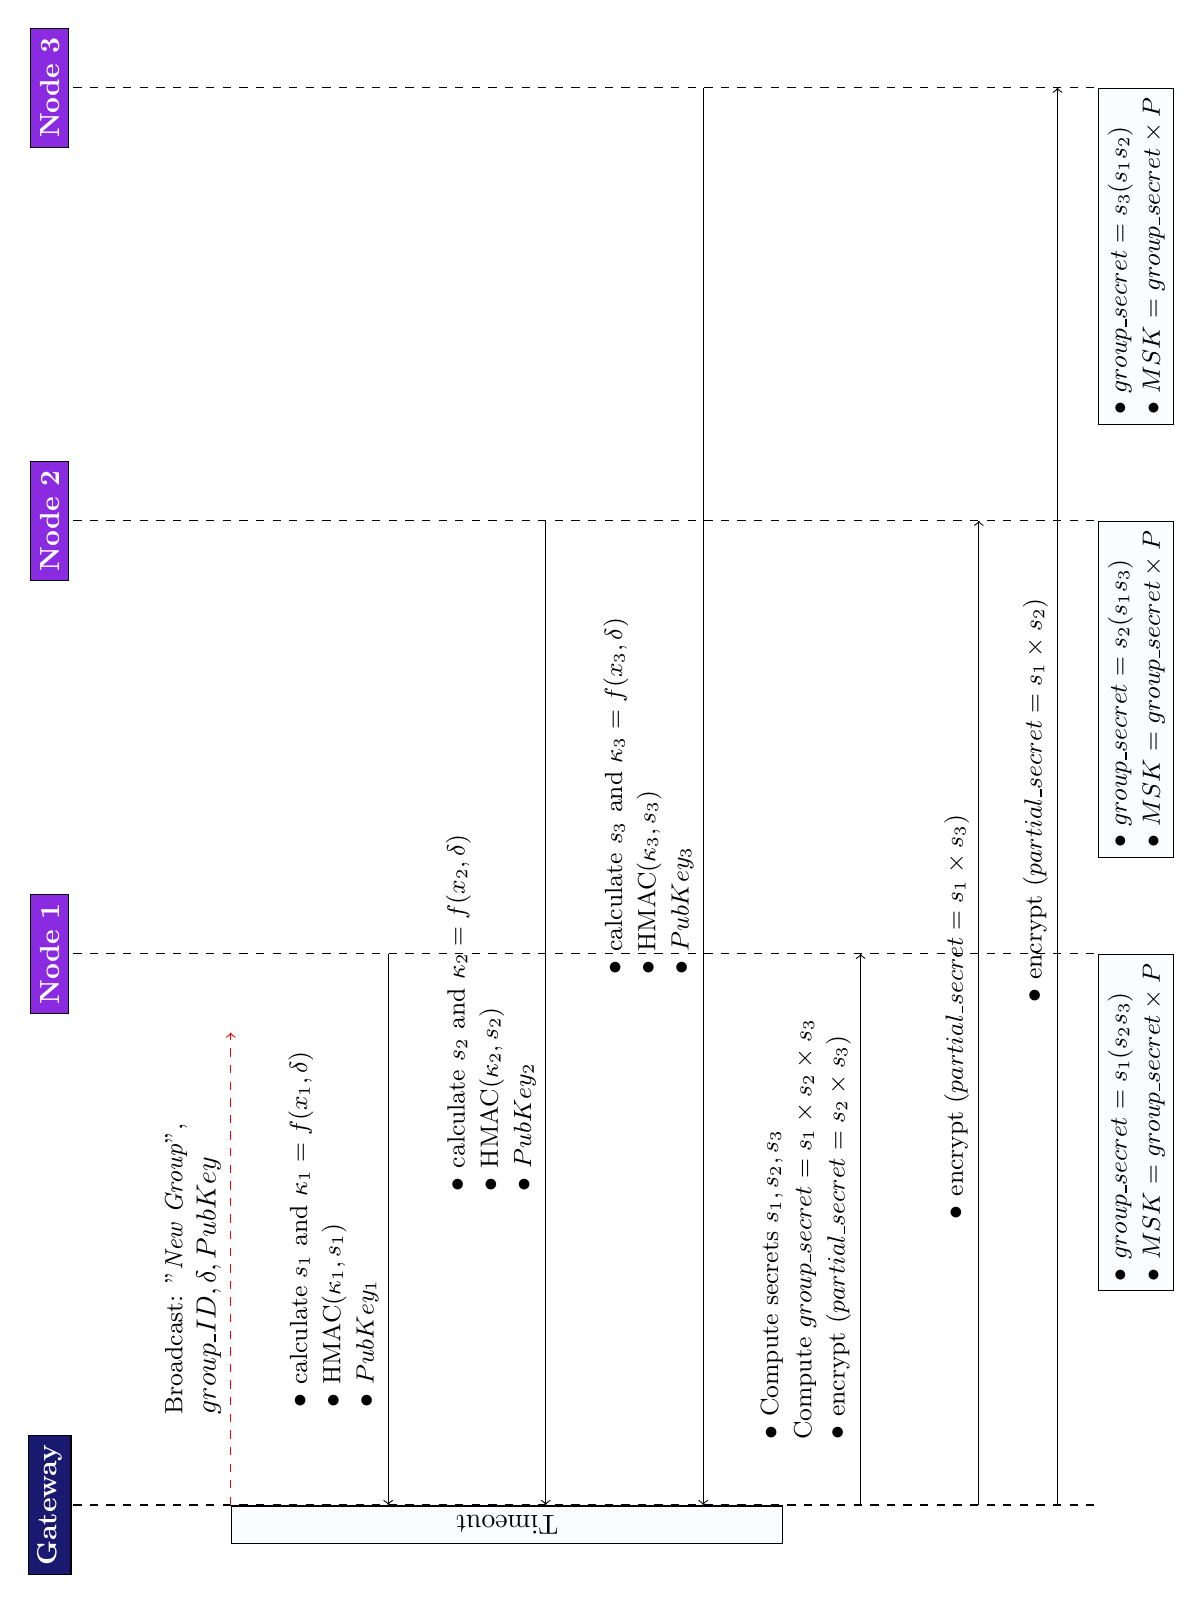
\begin{tikzpicture}[auto,rotate=90,transform shape]
    \draw (-8,0) -- (-8,-13)[dashed] (-1,0) -- (-1,-13)  (4.5,0) -- (4.5,-13)  (10,0) -- (10,-13);
    \node at (-8,.3) [draw,thin,fill=MidnightBlue, text=White]{\textbf{Gateway}};
    \node at (-1,.3) [draw,thin,fill=BlueViolet, text=White]{\textbf{Node 1}};
    \node at (4.5,.3) [draw,thin,fill=BlueViolet, text=White]{\textbf{Node 2}};
    \node at (10,.3) [draw,thin,fill=BlueViolet, text=White]{\textbf{Node 3}};
    \node at (-8.25,-2) [drawrect, rotate=90, fill= SkyBlue!5, minimum width=7cm]  { Timeout};
    \draw[->, dashed, draw=red] (-8,-2) -- node[midway,above,align=left] {
        \small Broadcast: "\textit{New Group}",\\$group\_ID, \delta , PubKey$ 
        } (-2,-2);
    \draw[<-] (-8,-4) -- node[midway,above,align=left] {
    $\bullet$ \small calculate  $s_1$ and  $\kappa_1 = f(x_1,\delta)$\\
    $\bullet$ \small HMAC($\kappa_1 , s_1$)\\
    $\bullet$ \small $PubKey_1$
    } (-1,-4);
    
    \draw[<-] (-8,-6) -- node[midway,above,align=left] {
    $\bullet$ \small calculate  $s_2$ and  $\kappa_2 = f(x_2,\delta)$\\
    $\bullet$ \small HMAC($\kappa_2 , s_2$)\\
    $\bullet$ \small $PubKey_2$
    } (4.5,-6);
    
    \draw[<-] (-8,-8) -- node[midway,above,align=left] {
    $\bullet$ \small calculate  $s_3$ and  $\kappa_3 = f(x_3,\delta)$\\
    $\bullet$ \small HMAC($\kappa_3 , s_3$)\\
    $\bullet$ \small $PubKey_3$
    } (10,-8);
    
    \draw[->] (-8,-10) -- node[midway,above,align=left] {
    $\bullet$ \small Compute secrets $s_1, s_2, s_3$ \\
    \small Compute $group\_secret = s_1 \times s_2 \times s_3$ \\
    $\bullet$ \small encrypt ($partial\_secret = s_2 \times s_3$)
    } (-1,-10);
    
    \draw[->] (-8,-11.5) -- node[midway,above,align=left] {
    $\bullet$ \small encrypt ($partial\_secret = s_1 \times s_3$)
    } (4.5,-11.5);
    
    \draw[->] (-8,-12.5) -- node[midway,above,align=left] {
    $\bullet$ \small encrypt ($partial\_secret = s_1 \times s_2$)
    } (10,-12.5);
    
    \node at (-1,-13.5) [draw,thin, align=left, anchor=east, fill= SkyBlue!5 ]{
    \small $\bullet$ $group\_secret = s_1 (s_2 s_3)$\\
    \small$\bullet$ $MSK = group\_secret  \times \mathbb{P}$};
    
    \node at (4.5,-13.5) [draw,thin, align=left, anchor=east, fill= SkyBlue!5 ]{
    \small$\bullet$ $group\_secret = s_2 (s_1 s_3)$\\
    \small $\bullet$ $MSK = group\_secret  \times \mathbb{P}$};
    
    \node at (10,-13.5) [draw,thin, align=left, anchor=east, fill= SkyBlue!5 ]{
    \small$\bullet$ $group\_secret = s_3 (s_1 s_2)$\\
    \small$\bullet$ $MSK = group\_secret \times \mathbb{P}$};
\end{tikzpicture}
\end{center}
\caption{Group Key Initialization: The figure shows the messages exchanged between G and three end nodes which replied to the join request before the
specified timeout.}
\label{fig_group_key}
\end{figure*}